%!TEX root = ../Thesis.tex

\chapter{Evaluation and optimization}
	During the course of creating the application we tried different approaches to several interim steps. In this chapter we discuss how using different algorithms yielded different results.

	\section{Dataset}
	In order to test and optimize our detector we created a set of 101 images and annotated them manually with the following information: each intersection on the board was marked with a point, either as an empty intersection, an intersection with a white piece on it or one occupied by a black piece. Also, the location of all pieces was marked with a circle, i.e. with a center and its approximate radius.

	To have an image set that covers as many possible game situations as possible we took pictures in three different lighting conditions and on different backgrounds. Each time we took images of an empty board without any pieces, a board with only some few images and a configuration as it often happens during endgame. That is, many pieces on the board and lots of them in a line.

	Each board configuration was photographed from different angles in $\varphi$ (azimuth) and $\theta$ (polar) direction and from two directions, i.e. facing the board from the side a player would and rotated by 90\textdegree~ as a third person would see the board.

	\begin{figure}
		\begin{subfigure}[b]{0.3\textwidth}
			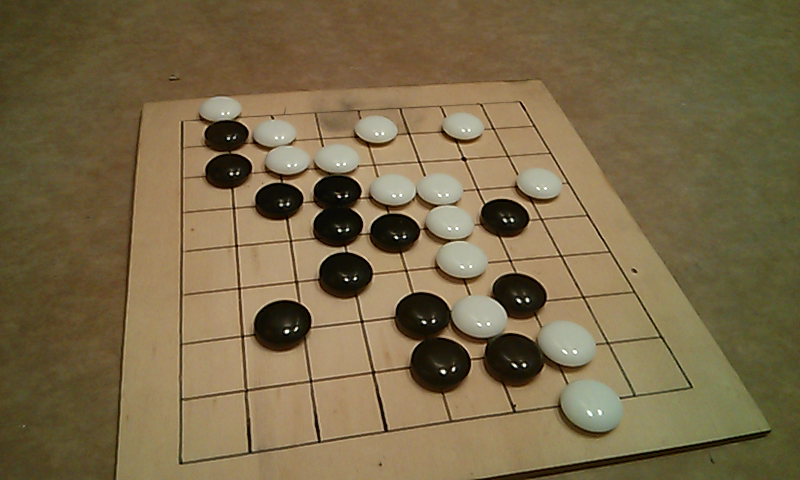
\includegraphics[width=\textwidth]{images/warmLight_many_leftMedium.png}
			\caption{Paper in warm light; camera left on medium height}
		\end{subfigure}
		~
		\begin{subfigure}[b]{0.3\textwidth}
				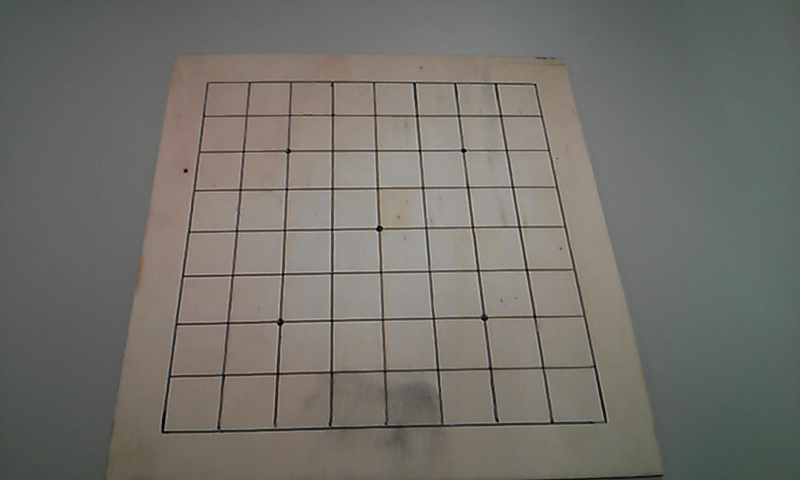
\includegraphics[width=\textwidth]{images/neonDesk_empty_centerAbove.png}
				\caption{Plain gray desk in neon light; camera centered high}
		\end{subfigure}
		~
		\begin{subfigure}[b]{0.3\textwidth}
				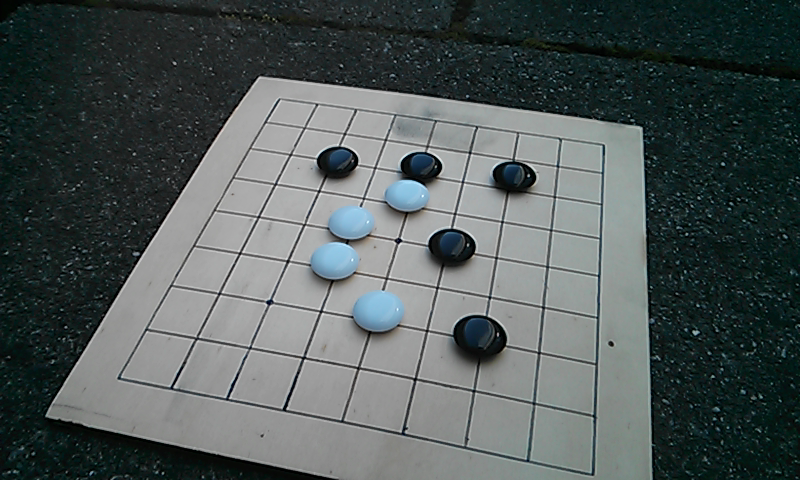
\includegraphics[width=\textwidth]{images/shadowStone_some_rightAbove.png}
				\caption{Dark stone surface in the shadow; camera right high}
		\end{subfigure}
		\\
		\begin{subfigure}[b]{0.3\textwidth}
				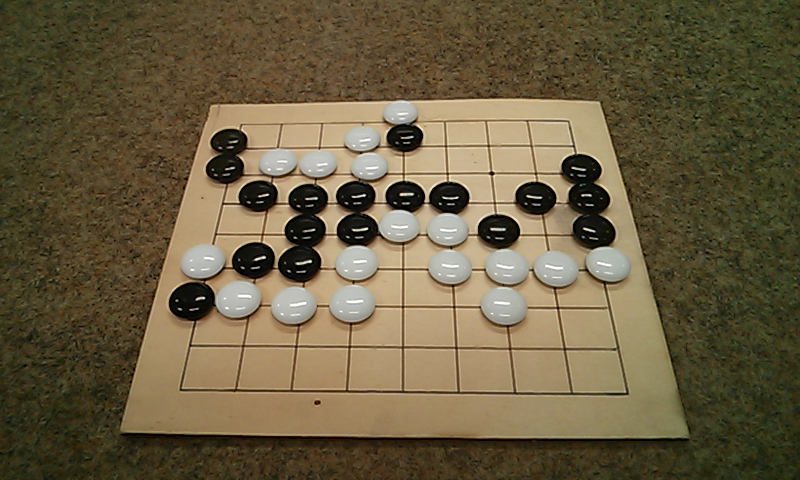
\includegraphics[width=\textwidth]{images/neonFloor_many_centerLow.png}
				\caption{Brown carpet in neon light; camera centered low}
		\end{subfigure}
		~
		\begin{subfigure}[b]{0.3\textwidth}
				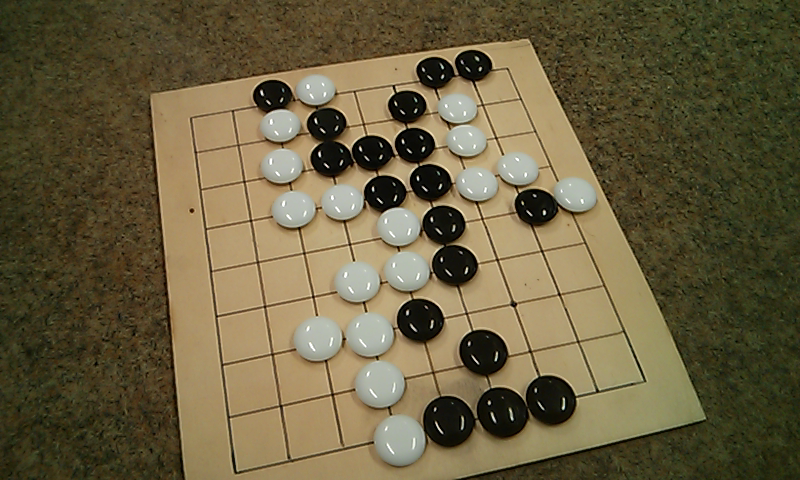
\includegraphics[width=\textwidth]{images/neonFloor_many_centerLow_rotated.png}
				\caption{Like (d) but from bystanders'	 perspective}
		\end{subfigure}
		~
		\begin{subfigure}[b]{0.3\textwidth}
			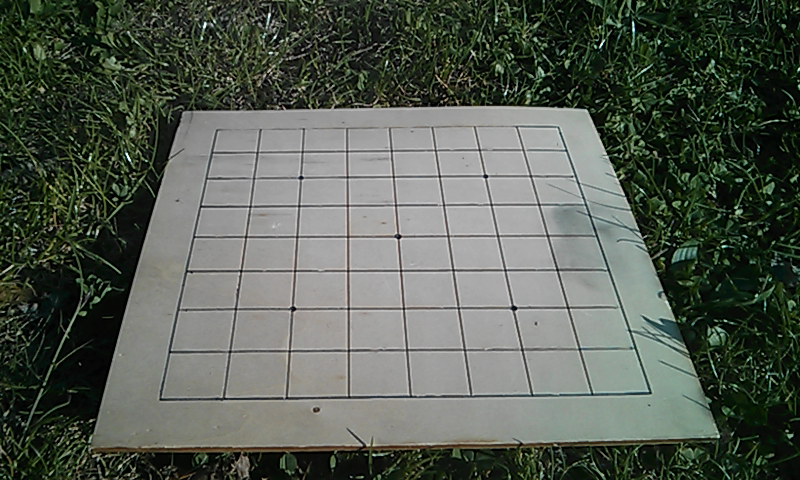
\includegraphics[width=\textwidth]{images/sunnyGrass_empty_centerLow.png}
			\caption{On grass in sunlight; camera centered low}
		\end{subfigure}

		\caption{Some examples of different lighting conditions, angles and backgrounds as well as different piece count}
		\label{fig:sampeImages}
	\end{figure}

	We ended up with: 29 images taken in cold neon light on a plain gray desk; 26 images taken in the same light on a textured, brown carpet; 25 images taken on a sunny day in the shadow on a stone surface; 17 images in warm artificial light on a textured paper background. Furthermore we have 5 images taken in the sun on an evening in which the board lay in grass. See \autoref{fig:sampeImages} for some examples from the image set.

	The images were taken by starting the app normally but then instead of starting detection saving the input image on the internal memory of the device. While in the beginning we saved images to png we later switched to persisting the images into yml format and retake the previous images. This has the advantage that we can be absolutely sure that the input to our test instances are the same as they would be on a phone, as no png coding and decoding takes place. Also we had problems in the beginning because OpenCV's image persisting function presumably does not recognize that the camera image is encoded in RGB (see \autoref{android-detector}), which lead to different results on our desktop hardware than on our Android phone.

	31 of the images were randomly chosen as a test set evenly spread over all lighting conditions as well as piece and angle configurations. The grass images were not part of the test set as they soon turned out to be very difficult. We included them in the training set, though. This set was used to improve our detector.

	To do so we assumed that there is a global maximum for the overall quality of results when adjusting parameters of the used algorithms. Even if this assumption were wrong we optimized for a local maximum. Then we tried manually to find roughly the optimal parameters for some randomly chosen images for every algorithm. Finally we adjusted them automatedly by brute forcely trying every combination of parameters in the vicinity of the manually chosen on every image on a cluster of 45 oktacore machines and checking the results against the annotations.






	\section{Visible intersections}
	%TODO: eigentlich ist visible intersections falsch, weil ja auch unsichtbare gematcht werden
	When evaluating the detection rate of visible intersections we first checked if the intersection was within the boundaries of the annotated board and a padding of 15 pixels. If not the intersection was considered uninteresting and did neither count positively nor negatively. If it was inside the board we searched the nearest annotated intersection for every detected one. If there was none within a range of 15 pixels the intersection was counted as a false positive. But if there was, then the annotated intersection was marked as detected and not considered as a possible match for other intersections. The threshold was chosen roughly as a quarter of the average distance between two intersections and a third of the diameter of a piece as measured in some sample images.

	%!TEX root = ../Thesis.tex

\begin{figure}
	\pgfplotsset{width=\textwidth, height=5.5cm, compat=1.11}
	\begin{subfigure}{\textwidth}
		\begin{tikzpicture}
			\begin{semilogyaxis}[
				ylabel={Intersections count},
				xlabel={Different parameter combinations},
				xtick style={draw=none},
				xticklabels={,,},
				axis x line=bottom,
				axis y line=left,
				legend style={at={(1,0.05)}, anchor=south east},
				xmin=0,
				ymin=0,
				xmax=610,
				ymax=6000
				]
				\draw[white!70!black, thin] ({rel axis cs:1,0}|-{axis cs:0,5670}) -- ({rel axis cs:0,0}|-{axis cs:0,5670});
				\draw[white!70!black, thin] ({rel axis cs:1,0}|-{axis cs:0,70}) -- ({rel axis cs:0,0}|-{axis cs:0,70});
				\draw[orange, thick] ({axis cs:381,5000}) -- ({axis cs:381,0}|-{rel axis cs:0,0});
				\draw[orange, thick] ({axis cs:0,5000}) -- ({axis cs:381,5000});

				\addplot[color=red, smooth]          table[x expr=\coordindex+1, y=matched, mark=none] {plots/lines_hough_part.csv};
				\addplot[color=red!40!black, smooth] table[x expr=\coordindex+1, y=wrong, mark=none] {plots/lines_hough_part.csv};

				\addlegendentry{Sum of true positives on all images}
				\addlegendentry{Sum of all false positives on all images}
			\end{semilogyaxis}
		\end{tikzpicture}
		\vspace{-20pt}
		\caption{Representative subset of 605 combinations of 60481 tested for the Houghline detector}
		\label{fig:linesTraining-hough}
	\end{subfigure}
	\vspace{20pt}

	\begin{subfigure}{\textwidth}
		\begin{tikzpicture}
			\begin{semilogyaxis}[
				ylabel={Intersections count},
				xlabel={Different parameter combinations},
				xtick style={draw=none},
				xticklabels={,,},
				axis x line=bottom,
				axis y line=left,
				legend style={at={(1,0.05)}, anchor=south east},
				xmin=0,
				ymin=0,
				xmax=610,
				ymax=6000
				]
				\draw[white!70!black, thin] ({rel axis cs:1,0}|-{axis cs:0,5670}) -- ({rel axis cs:0,0}|-{axis cs:0,5670});
				\draw[white!70!black, thin] ({rel axis cs:1,0}|-{axis cs:0,70}) -- ({rel axis cs:0,0}|-{axis cs:0,70});
				\draw[orange, thick] ({axis cs:158,1175}) -- ({axis cs:158,0}|-{rel axis cs:0,0});
				\draw[orange, thick] ({axis cs:0,1175}) -- ({axis cs:158,1175});

				\addplot[color=blue, smooth]          table[x expr=\coordindex+1, y=matched, mark=none, smooth,] {plots/lines_lsd_part.csv};
				\addplot[color=blue!40!black, smooth] table[x expr=\coordindex+1, y=wrong, mark=none, smooth, blue] {plots/lines_lsd_part.csv};

				\addlegendentry{Sum of true positives on all images}
				\addlegendentry{Sum of all false positives on all images}
			\end{semilogyaxis}
		\end{tikzpicture}
		\vspace{-20pt}
		\caption{Representative subset of 605 combinations of 58321 tested for the LSD detector.}
		\label{fig:linesTraining-lsd}
	\end{subfigure}
	\vspace{20pt}

	\begin{subfigure}{\textwidth}
		\begin{tikzpicture}
			\begin{semilogyaxis}[
				ylabel={Intersections count},
				xlabel={Different parameter combinations},
				xtick style={draw=none},
				xticklabels={,,},
				axis x line=bottom,
				axis y line=left,
				legend style={at={(1,0.05)}, anchor=south east},
				xmin=0,
				ymin=0,
				xmax=610,
				ymax=15000
				]
				\draw[white!70!black, thin] ({rel axis cs:1,0}|-{axis cs:0,5670}) -- ({rel axis cs:0,0}|-{axis cs:0,5670});
				\draw[white!70!black, thin] ({rel axis cs:1,0}|-{axis cs:0,70}) -- ({rel axis cs:0,0}|-{axis cs:0,70});
				\draw[orange, thick] ({axis cs:117,215}) -- ({axis cs:117,0}|-{rel axis cs:0,0});
				\draw[orange, thick] ({axis cs:0,215}) -- ({axis cs:117,215});

				\addplot[color=green, smooth]          table[x expr=\coordindex+1, y=matched, mark=none, smooth,] {plots/intersects_fast_part.csv};
				\addplot[color=green!40!black, smooth] table[x expr=\coordindex+1, y=wrong, mark=none, smooth, blue] {plots/intersects_fast_part.csv};

				\addlegendentry{Sum of true positives on all images}
				\addlegendentry{Sum of all false positives on all images}
			\end{semilogyaxis}
		\end{tikzpicture}
		\vspace{-20pt}
		\caption{Representative subset of 605 combinations of 1440 tested for the FAST detector}
		\label{fig:linesTraining-fast}
	\end{subfigure}

	\caption{The x-axis shows different combinations of parameters that we have evaluated. On the y-axis the true positives, false positives, totally available intersections (upper gray line) and number of analyzed images (lower gray line) per combination can be seen. The x-axis does not imply any order of the tested combinations; results have been simply sorted after number of correct intersections. We chose the parameter combination with the highest true positive rate whilst less false positives than evaluated files (orange line)}
	\label{fig:linesTraining}
\end{figure}


	\subsection{Optimizations on the training set}
	While optimizing the parameters used in our algorithm, we measured the quality as the ratio of detected to undetected intersections, also considering the number of false positives. Traditionally one would calculate some ratio of true positives to false positives. However none of the usual measurement methods shows us a clear indicator what combinations of parameters to use, so we devised the following metric: We sorted the results by the number of correctly matched intersections and chose the highest one where the number of false positives was lower or equal than the number of images recognized ($|false\_positives| \leq |input\_images|$, i.e. statistically maximal one false positive per image). This is shown (albeit on a representative subset of all tested parameter combinations) in \autoref{optimizationlinesCorrectness}, where the parameters we chose is marked in orange.

	\subsubsection{HOUGH}
	In comparison to the other algorithms detecting the lines using Hough transformation performs best quality-wise. As \autoref{fig:houghCorrectness} shows, we still had to compromise when choosing the final parameter set. The one we chose as noted above resulted in 89.67\% (5084 out of 5670) correct detection rate in our training set, with a total of 68 incorrect intersections (0.01199\% of available intersections).

	The graphic shows also that that the quality of the line detection does not depend very much on the parameters used: there's only a few parameter combinations that yield very poor results and hardly any that results in finding no intersection at all. As would be expected the average number of false positives rises with the percentage of correctly found intersections. Luckily, there is enough variance yet that even at a high detection rate we can find entries with on average less than one false intersection per image.

	\subsubsection{LSD}
	As noted in \autoref{detector-visible-lsd} the Line Segment Detector needs significant postprocessing to give any reasonable results. Still it is easily outperformed by the variant using hough transformation. In \autoref{fig:linesTraining-lsd} it can easily be seen that the amount of false positives does not go below the amount of input images when roughly a quarter of all available intersections should be detected. Furthermore the average ratio of correct results to false positives is nearly over all combinations worse than its hough counterpart's. Only in the segment where both detect nearly 100\% of all correct intersections. The total number of wrong intersections ranges in the thousands here, though, making this segment unusable for the application.

	We can expect the detector to perform significantly worse as the chosen parameter combination performs at a detection rate of only 20.53\% (1164 out of 5670) with 69 false positives. To achieve a detection rate similar to the one of the hough detector we would have to accept more than 10 false positives per image.
	%TODO: was, wenn gras ausgenommen wird?

	\subsubsection{FAST}
	Even worse performs the FAST corner detector when used for detection of the intersections. It is the only detector that resulted in more false positives than correct intersections in some combination. The ratio of false positives to correct intersections is in no combination better than the of the intersections of lines detected using LSD or Hough transformation.

	The chosen parameter combination yields a mere 2.7\% 155 correctly detected intersections with 70 wrongly placed ones. Overall the detector seems to stick too much to the lines themselves and places many intersections around them and at the border of the black pieces. %nonmax suppression ist egal erwaehnen?

	\subsection{Performance on the testing set}
	\subsubsection{HOUGH}
	The hough detector produces quite good results in the test set. Those images where no (on the left in \autoref{fig:linesTest-hough}) hardly any pieces lie on the board are detected de facto perfectly. It does have some issues with boards with pieces on them and drops significantly (to about 60\% of the performance without pieces) when there are many pieces on the board (on the right in \autoref{fig:linesTest-hough}). This was to be expected, though, and the performance is still better compared with the other two algorithms.

	\begin{table}[b]
		\begin{tabular}{|r|r||>{\bfseries}c|c|c|}
			\cline{3-5}
		    \multicolumn{2}{c|}{}											 		& Hough 	& LSD 		& FAST     \\
			\cline{3-5}
			\hline
			\multirow{2}{*}{No pieces on the board}   		& True positive rate 	& 100\% 	& 30.3\%  	& 0.685\%  \\
			%
															& Precision			 	& 99.4\% 	& 94.2\%  	& 83.3\%  \\
			%																					  245/260	  5/6
			\hline
			\multirow{2}{*}{Some pieces on the board (7-13)}& True positive rate 	& 95.6\% 	& 11.4\% 	& 1.97\%   \\
			%
															& Precision 			& 98.6\% 	& 91.2\%  	& 53.3\%  \\
			%																					  114/125	  16/30
			\hline
			\multirow{2}{*}{Many pieces (27-34)} 			& True positive rate 	& 58.6\% 	& 9.02\% 	& 3.80\%   \\
			%
															& Precision			 	& 95.5\% 	& 94.0\%  	& 68.8\%  \\
			%																					  95/101	  33/48
			\hline
		\end{tabular}
		\caption{Quality of the tested algorithms on our test set. The hough transformation based algorithm dominates all categories.}
		\label{tab:linesTest}
	\end{table}

	\subsubsection{LSD}
	As was to be expected from the data of our training set the Line Segment Detector performed significantly worse than the Hough lines detector. The relative performance was actually still lower on our testing set than on our training set, where it reached 22\% of the quality of the hough detector, while on our testing data it could only achieve 20\% -- and that is only looking at the true positive rate. In total it matched 18\% of the available intersections. We can see that the precision ranks lower, too, and that it deals less well with pieces on the board than the first examined algorithm (its true positive rate sinks to one third when there are lots of pieces on the board compared to when there are none).

	\subsubsection{FAST}
	The corner detector based approach obviously does not yield results which justify further analysis. Interestingly, though, the percentage of correctly detected intersections rises with the number of pieces on the board. This might be because the white pieces reduce the amount of visible intersections making it more probable for a keypoint to lie on one, when being placed along visible edges.

	%!TEX root = ../Thesis.tex

\begin{figure}
	\pgfplotsset{width=\textwidth, height=5cm, compat=1.11}
	\begin{subfigure}{0.32\textwidth}
		\begin{tikzpicture}
			\begin{axis}[
				xticklabels={,,},
				axis x line=bottom,
				axis y line=left,
				xmin=0,
				ymin=0,
				xmax=32,
				ymax=1
				]
				\draw[gray] ({rel axis cs:1,0}|-{axis cs:0,81}) -- ({rel axis cs:0,0}|-{axis cs:0,81});

				\addplot[only marks, mark=*, mark options={scale=1.1, fill=red!40!black}]
					table[x expr=\coordindex+1, y expr=\thisrow{matched}/(\thisrow{matched}+\thisrow{wrong})] {plots/lines_hough_testSet.csv};
				\addplot[only marks, mark=*, mark options={scale=1.1, fill=red}]
					table[x expr=\coordindex+1, y expr=\thisrow{matched}/81] {plots/lines_hough_testSet.csv};
			\end{axis}
		\end{tikzpicture}
		\caption{Results of the Hough transformation detector}
		\label{fig:linesTest-hough}
	\end{subfigure}
	\hfill
	\begin{subfigure}{0.32\textwidth}
		\begin{tikzpicture}
			\begin{axis}[
				xticklabels={,,},
				axis x line=bottom,
				axis y line=left,
				xmin=0,
				ymin=0,
				xmax=32,
				ymax=1
				]
				\draw[gray] ({rel axis cs:1,0}|-{axis cs:0,81}) -- ({rel axis cs:0,0}|-{axis cs:0,81});

				\addplot[only marks, mark=*, mark options={scale=1.1, fill=blue!40!black}]
					table[x expr=\coordindex+1, y expr=\thisrow{matched}/(\thisrow{matched}+\thisrow{wrong})] {plots/lines_lsd_testSet.csv};
				\addplot[only marks, mark=*, mark options={scale=1.1, fill=blue}]
					table[x expr=\coordindex+1, y expr=\thisrow{matched}/81] {plots/lines_lsd_testSet.csv};
			\end{axis}
		\end{tikzpicture}
		\caption{Results of the LSD detector}
		\label{fig:linesTest-lsd}
	\end{subfigure}
	\hfill
	\begin{subfigure}{0.32\textwidth}
		\begin{tikzpicture}
			\begin{axis}[
				xticklabels={,,},
				axis x line=bottom,
				axis y line=left,
				xmin=0,
				ymin=0,
				xmax=32,
				ymax=1
				]
				\draw[gray] ({rel axis cs:1,0}|-{axis cs:0,81}) -- ({rel axis cs:0,0}|-{axis cs:0,81});

				\addplot[only marks, mark=*, mark options={scale=1.1, fill=green!40!black}]
					table[x expr=\coordindex+1, y expr=\thisrow{matched}/(\thisrow{matched}+\thisrow{wrong})] {plots/intersections_fast_testSet.csv};
				\addplot[only marks, mark=*, mark options={scale=1.1, fill=green}]
					table[x expr=\coordindex+1, y expr=\thisrow{matched}/81] {plots/intersections_fast_testSet.csv};
			\end{axis}
		\end{tikzpicture}
		\caption{Results of the corner detector}
		\label{fig:linesTest-fast}
	\end{subfigure}

\caption{True positive rate (light color filled circles) and precision (dark color filled circles) per image in our test set.}
\label{fig:linesTest}
\end{figure}

	\clearpage





	\section{Occluded intersections}
	\subsection{Optimizations on the training set}
	We optimized the parameters for thresholding and detecting light and dark pieces separately for both detection methods. We chose the final parameter set like we did for the line detection algorithms by sorting after true positive rate and selecting the best scoring algorithm below a specific threshold on false positives. We set the false positive threshold a lot lower, though, at a maximum of seven false positives for either color. That is because we found that wrongly classified pieces tended to have a greater impact on detection quality than false positives in the line detection step. Both algorithms still performed good enough to provide a significant amount of additional intersections.

	Due to how we optimized our parameters we could not adjust the thresholding values for both methods or even all parameters at once. Therefore we first set the contours to very general settings and used it to find a parameter set of the thresholding step where there were not too many false positives and the detection rate was not too low.
	%TODO: nochmal auf optimierte erkenner parameter optimieren

	\subsubsection{Contours}
	As described in \autoref{detector-occluded-contours} we selected rectangles around contours of blobs in the thresholded images when they were roughly quadratic. This works surprisingly well and we believe it could be improved still to perform as good as hough circle detection or even better, by using rotated rectangles. The chosen parameters yielded 84.23\% (438 of 520) detection rate with 3 false positives on the white pieces and 61.12\% (316 of 517) detection rate with 7 false positives on the black pieces. When added together this results in a 72.71\% (754 of 1037) detection rate with 10 false positives. Another optimization run on the threshold values did not increase the detection rate significantly.

	\subsubsection{Hough}
	The more obvious approach is to use hough circle detection to locate the pieces as mentioned in \autoref{detector-occluded-hough}. This approach correctly detected 78.27\% (407 of 520) with 5 false positives of the white pieces and 69.05\% (357 of 517) with 6 false positives of the black pieces. Summed up this is a 73.67\% (764 of 1037) detection rate with 11 false positives.

	\subsection{Performance on the testing set}
	%!TEX root = ../Thesis.tex

\begin{figure}
	\pgfplotsset{width=\textwidth, height=5cm, compat=1.11}
	\begin{subfigure}{0.45\textwidth}
		\begin{tikzpicture}
			\begin{axis}[
				xticklabels={,,},
				axis x line=bottom,
				axis y line=left,
				ylabel={TPR \& Precision},
				xlabel={Tokens on the board},
				xmin=0,
				ymin=0,
				xmax=32,
				ymax=1
				]
				\draw[gray] ({rel axis cs:1,0}|-{axis cs:0,81}) -- ({rel axis cs:0,0}|-{axis cs:0,81});

				\addplot[only marks, mark=*, mark options={scale=1.1, fill=orange!40!black}]
					table[x expr=\coordindex+1, y expr=\thisrow{matched}/(\thisrow{matched}+\thisrow{wrong})] {plots/pieces_contour_testSet.csv};
				\addplot[only marks, mark=*, mark options={scale=1.1, fill=orange}]
					table[x expr=\coordindex+1, y expr=\thisrow{matched}/\thisrow{available}] {plots/pieces_contour_testSet.csv};
			\end{axis}
		\end{tikzpicture}
		\caption{Results of the contour based detector}
		\label{fig:piecesTest-contour}
	\end{subfigure}
	\hfill
	\begin{subfigure}{0.45\textwidth}
		\begin{tikzpicture}
			\begin{axis}[
				xticklabels={,,},
				axis x line=bottom,
				axis y line=left,
				ylabel={TPR \& Precision},
				xlabel={Tokens on the board},
				xmin=0,
				ymin=0,
				xmax=32,
				ymax=1
				]
				\draw[gray] ({rel axis cs:1,0}|-{axis cs:0,81}) -- ({rel axis cs:0,0}|-{axis cs:0,81});

				\addplot[only marks, mark=*, mark options={scale=1.1, fill=magenta!40!black}]
					table[x expr=\coordindex+1, y expr=\thisrow{matched}/(\thisrow{matched}+\thisrow{wrong})] {plots/pieces_hough_testSet.csv};
				\addplot[only marks, mark=*, mark options={scale=1.1, fill=magenta}]
					table[x expr=\coordindex+1, y expr=\thisrow{matched}/\thisrow{available}] {plots/pieces_hough_testSet.csv};
			\end{axis}
		\end{tikzpicture}
		\caption{Results of the hough transformation detector}
		\label{fig:piecesTest-hough}
	\end{subfigure}

\caption{True positive rate (light color filled circles) and precision (dark color filled circles) per image in our test set.}
\label{fig:piecesTest}
\end{figure}

	Interestingly the contour based approach yields better results when there are less pieces on the board. This is probably due to how the algorithm handles two adjacent pieces which are connected. Not all of those are correctly split into two pieces and thus discarded. If this could be improved it would probably outperform its hough based counterpart.

	When summing up the results both approaches, both perform equally well on our testing set as \autoref{tab:piecesTest} shows.
	\begin{table}[bh]
		\begin{tabular}{|r|r||c|c|}
			\cline{3-4}
		    \multicolumn{2}{c|}{}											 		& Contour 	& HOUGH\\
			\cline{3-4}
			\hline
			\multirow{2}{*}{No pieces on the board}   		& True positive rate 	& N/A 		& N/A  \\
															& Precision			 	& 1 false positive 		& \bf{N/A} \\
			\hline
			\multirow{2}{*}{Some pieces on the board (7-13)}& True positive rate 	& \bf{86.7\%} 	& 75.90\% \\
			%																		  72/83 		  63/83
															& Precision 			& 98.6\% 		& \bf{100\%} \\
			%																		  72/73 		  63/63
			\hline
			\multirow{2}{*}{Many pieces (27-34)} 			& True positive rate 	& 40.0\% 		& \bf{70.6\%} \\
			%																		  243/357		  252/357
															& Precision			 	& 99.2\% 		& 99.2\% \\
			%																		  246/248 		  252/254
			\hline
			\hline
			\multirow{2}{*}{Total}				 			& True positive rate 	& 71.6\% 		& 71.6\% \\
			%																		  315/440		  315/440
															& Precision			 	& 97.8\% 		& \textbf{99.3}\% \\
			%																		  315/322 		  315/317
			\hline
		\end{tabular}
		\caption{Quality of the tested algorithms on our test set. When there are no pieces on the board neither rate can be calculated (TPR divides by zero, Precision becomes zero)}
		\label{tab:piecesTest}
	\end{table}





	\section{Speed on an Android device}
	\subsection{Getting a baseline}
	\subsection{Comparing runtime of different approaches}
	\pgfplotstableread[header=false]{
	345.24 	{Hough lines}
	168.46	{LSD lines}
	322.58	{Hough pieces}
	249.69	{Contour pieces}
	51.33 {Framework}
	}\datatable
	\pgfplotsset{
    select row/.style={
        x filter/.code={\ifnum\coordindex=#1\else\def\pgfmathresult{}\fi}
    }
}
	\begin{figure}
		\pgfplotsset{width=\textwidth, height=5cm, compat=1.11}
		\begin{tikzpicture}
			 \begin{axis}[
				        xbar,
				        bar shift=0pt,
				        xmin=0,
				        xmax=400,
				        ytick={0, 1, 2.5, 3.5, 5},
				        yticklabels from table={\datatable}{1},
				        xmajorgrids = true,
				        width=12cm,
				        height=5.5cm,
				        xlabel={Time in ms},
				        nodes near coords, nodes near coords align={horizontal},
				  ]

				\addplot[fill=gray] table [select row=4, y expr=5] {\datatable};
				\addplot[fill=orange] table [select row=3, y expr=3.5] {\datatable};
				\addplot[fill=magenta] table [select row=2, y expr=2.5] {\datatable};
				\addplot[fill=blue] table [select row=1, y expr=1] {\datatable};
				\addplot[fill=red] table [select row=0, y expr=0] {\datatable};
			  \end{axis}
		\end{tikzpicture}
		\caption{TODO}
		\label{fig:timeEvaluation}
	\end{figure}



	\section{Pre- and postprocessing}

	\subsection{Rectifying perspective distortion}
	The camera moves only slightly when hand-held or not at all when put on some kind of stand. Thus it should be feasible to use the orientation of the board in a previous frame to correct the orientation in the current frame. This information must only be discarded when the camera moves drastically or when the result in the current frame is very bad due to the correction. Therefore we enabled the detector to receive a transformation matrix, apply it to the input image before any operation happens and transform the results back after all detection has taken place.

	The source of the transformation is the inverse transformation matrix determined by the RANSAC step in our detection pipeline. This automatically incorporate lens distortion, too.

	We did not have video test data so to test the first approach we instead fed the transformation matrix back into a second run on the same image. Assuming the location of the camera does not change too much during two frames this substitution can be made. The first impression of using doing so were pretty promising. The images were transformed well and seemed to be taken from directly above the board.

	However having reached near-perfect accuracy on the test set by optimizing for images taken from an angle the results were poorer than before. This does not mean that the step is a failure, though, but simply that the optimized parameters for the other pipeline steps are very well fitted to the given task. When researching the task further it might be a good idea to incorporate this preprocessing step upfront.

	\subsection{Removing large outliers during detection}
	When testing our pipeline on an actual android device we recognized that two successive frames could yield completely different results. Mostly the differences were marginal but sometimes between two correctly classified images there was one which was detected very poorly.

	\subsubsection{Moving average over intersection results}
	To mitigate the effects of those frames we tried applying a moving average over the intersections. The previously detected intersection counted 75\% while those from the current image contributed only 25\%, i.e. $I_t = \frac{1}{4}I + \frac{3}{4}I_{t-1}$.

	While this approach removed large outliers from the detection result on wrongly classified images, it also led to worse results. That is due to large errors having such influence that the result would be skewed for several frames to come.

	\subsubsection{Filtering obviously incorrect detection results}
	Our next approach was to filter out obviously wrong classified detection results. We considered a result to be wrong when at least one intersection lay outside of the image or if the distance between two intersections was smaller than five pixels. We then marked the whole board as unclassified (i.e. neither black, white or empty) and did not count these steps when calculating the average over time as mentioned in \autoref{android-detector}.

	After implementing this approach we hardly ever saw incorrect results when capturing a game and so we kept it in our final application.





	\section{Overall performance and live experiences}
	We furthermore chose to use Houghlines as it was the only well-performing line detector. For the detection of pieces we used the contour based algorithm due to its speed advantages for the final application as it was released to the Google Play Store\footnote{It can be installed at \url{https://play.google.com/store/apps/details?id=de.t_animal.goboardreader}}.

	... === TODO === ...

	We were contempt with these results and tried to max out the amount of pieces we could place on the board to see how well the algorithm performed under extreme circumstances. The result was pretty good. Detection was possible until the board was nearly completely covered in pieces. We then put a piece on each intersection in a checkerboard like pattern -- alternating black and white. Even this completely abnormal configuration could be detected with near 100\% accuracy as \autoref{fig:android_perfect_recognition} shows. The results were very unstable, though. That means between a correctly classified frame lay several discarded ones, which did not contribute to the detection result but prolonged the detection time.

	\begin{figure}[h]
		\center
		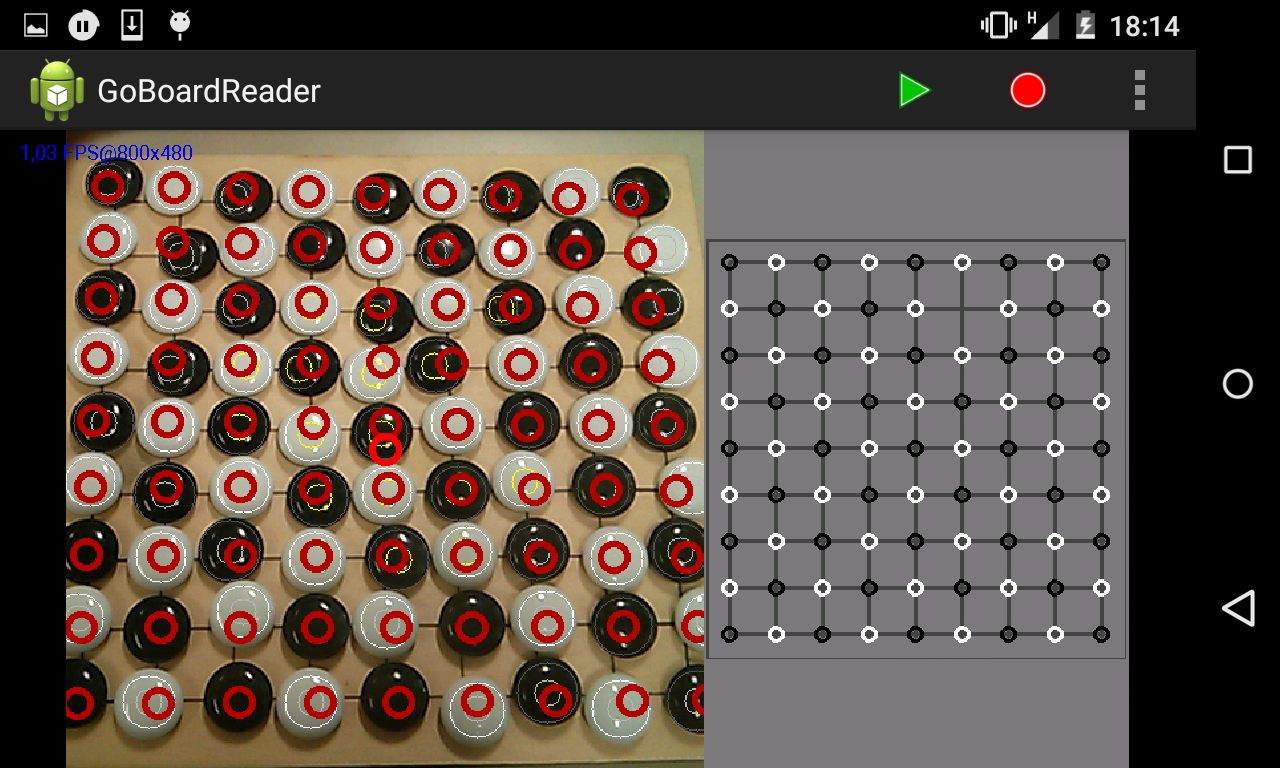
\includegraphics[width=0.7\textwidth]{images/android_perfect_recognition.png}
		\caption{The performance on a hand-held Nexus 4 and a completely covered board}
		\label{fig:android_perfect_recognition}
	\end{figure}
